\documentclass[letterpaper]{article}
\usepackage[margin=1in, bottom=1.25in, footskip=0.5in]{geometry}
\usepackage[utf8]{inputenc}
\usepackage[IL2]{fontenc}
\usepackage{lmodern}
\usepackage[slovak]{babel}

\usepackage{indentfirst}
\usepackage[dvipsnames]{xcolor}
\usepackage{color}

\definecolor{bluekeywords}{rgb}{0,0,1}
\definecolor{greencomments}{rgb}{0,0.5,0}
\definecolor{redstrings}{rgb}{0.64,0.08,0.08}
\definecolor{xmlcomments}{rgb}{0.5,0.5,0.5}
\definecolor{types}{rgb}{0.17,0.57,0.68}

\usepackage{listings}
\lstset{language=[Sharp]C,
	tabsize=4,
	captionpos=b,
	%numbers=left, %Nummerierung
	%numberstyle=\tiny, % kleine Zeilennummern
	frame=lines, % Oberhalb und unterhalb des Listings ist eine Linie
	showspaces=false,
	showtabs=false,
	breaklines=true,
	showstringspaces=false,
	breakatwhitespace=true,
	escapeinside={(*@}{@*)},
	commentstyle=\color{greencomments},
	morekeywords={partial, var, value, get, set},
	keywordstyle=\color{bluekeywords},
	stringstyle=\color{redstrings},
	basicstyle=\linespread{1}\ttfamily\small,
}

\setlength{\parindent}{2em}
\setlength{\parskip}{1em}

\linespread{1.25}

\let\stdsection\section							% 
\renewcommand\section{\newpage\stdsection}		% nová sekcia na novej strane

\usepackage{fancyvrb}
\usepackage{graphicx}

\title{Semestrálna práca}
\author{Andrej Rábek}

\begin{document}
	\begin{titlepage}
		\begin{center}
			\vspace*{1cm}
			
			\Huge
			\textbf{Simulácia\\vakcinačného centra}
			
			\LARGE
			\textbf{Agentovo-orientovaná simulácia}
			
			\vspace{1.5cm}
			
			\textbf{Andrej Rábek}\\
			5ZIS12
			
			\vfill
			
			Semestrálna práca 3
			
			\vspace{0.8cm}
			
			\Large
			Fakulta riadenia a informatiky\\
			Žilinská univerzita v Žiline\\
			\today
			
		\end{center}
	\end{titlepage}
	
	\tableofcontents
	
	\section{Zadanie}
	
	Pre existujúce vakcinačné centrum, je potrebné vypracovať simulačnú štúdiu a preveriť potrebu jeho budúceho rozšírenia vzhľadom na očakávané zvýšenie dodávok vakcín. 
	
	Do vakcinačného centra prichádzajú vopred objednaní ľudia. Po príchode sa každý musí najskôr zaregistrovať. Osoba vstúpi do registračnej miestnosti a náhodne si vyberie jedného z voľných \textbf{administratívnych pracovníkov}. Ak žiadny pracovník nie je voľný, tak osoba čaká v rade (ľudia vytvárajú jediný rad a prvý v rade si vyberá z dostupných pracovníkov). \textbf{Administratívny pracovník} skontroluje doklad totožnosti a objednanie danej osoby na vakcináciu. Taktiež pomôže s vyplnením krátkeho dotazníka. 
	
	Po skončení registrácie sa osoba presunie na lekárske vyšetrenia do vedľajšej miestnosti. Osoba si náhodne vyberie jedného z voľných \textbf{lekárov}. Ak žiadny lekár nie je voľný, tak osoba čaká v rade (ľudia vytvárajú jediný rad a prvý v rade si vyberá z dostupných lekárov). \textbf{Lekár} preberie s pacientom jeho zdravotný stav, poučí pacienta o rizikách očkovania, zaregistruje do systému vakcínu a jej šaržu, ktorá bude aplikovaná. Na konci podpíše pacient informovaný súhlas s vykonaním očkovania príslušnou vakcínou.
	
	Následne sa osoba presunie na výkon očkovania do ďalšej miestnosti. Osoba si náhodne vyberie jednu z voľných \textbf{zdravotných sestier}. Ak žiadna sestra nie je voľná, tak osoba čaká v rade (ľudia vytvárajú jediný rad a prvý v rade si vyberá z dostupných sestier). \textbf{Zdravotná setra} aplikuje očkovaciu látku.
	
	Nakoniec sa osoba presunie do čakárne, kde zotrvá lekárom stanovený čas, pričom sa sleduje jej zdravotný stav.
	
	\textbf{Zdravotné sestry} zabezpečujú očkovanie, ale aj prípravu očkovacej látky a jej natiahnutie do injekčných striekačiek. Každá sestra má k dispozícii miesto na uloženie \textbf{dvadsiatich striekačiek} s očkovacou látkou. V prípade, že niektorá sestra už nemá k dispozícii žiadnu injekčnú striekačku s pripravenou vakcínou prestane s očkovaním (pacienti k nej už neprichádzajú) a ide si pripravovať ďalšie očkovacie dávky. \textbf{Presunie sa do vedľajšej miestnosti} s chladiacim zariadením, kde si postupne naplní 20 injekčných striekačiek očkovacou látkou. Následne sa presunie naspať do miestnosti, kde prebieha očkovanie a pokračuje v práci. Súčasne si môžu injekcie pripravovať \textbf{najviac 2 sestry}, ostatné sestry musia v tomto prípade počkať v rade.
	
	Pracovníci si musia spraviť obednú prestávku, avšak aj v čase obedov musí vakcinačné centrum fungovať. Pre každú skupinu pracovníkov je vyhradený osobitný čas na obed. Pre administratívnych pracovníkov je stanovený čas od \textbf{11:00}, pre lekárov od \textbf{11:45} a pre sestry od \textbf{13:30}. Súčasne môže obedovať \textbf{najviac polovica} pracovníkov z danej skupiny. Keď príde čas obeda určený pre danú skupinu pracovníkov, tak sa najviac polovica z tých, ktorí nepracujú vyberie do jedálne. Ostatní pokračujú v práci. Vždy keď sa vráti nejaký pracovník z obeda môže odísť na obed ďalší pracovník. Teda v prípade, že pracovník skončí obsluhu nejakej osoby, ešte neobedoval a je čas väčší ako čas na obed môže sa presunúť na obed (stále musí byť dodržané pravidlo, že súčasne môže obedovať najviac polovica pracovníkov z danej skupiny). 
	
	\noindent Pre vypracovanie simulačnej štúdie sú k dispozícii nasledujúce informácie:
	\begin{itemize}
		\item Vakcinačné centrum pracuje od 8:00 do 17:00.
		\item Pacienti sú objednávaní po jednej minúte, pričom všetky termíny sú obsadené. Na jeden deň je teda objednaných 540 pacientov. Predpokladajme, že pacienti prichádzajú v čase na ktorý sú objednaní.
		\item Bolo zistené, že počet pacientov, ktorý sa denné nedostavia a nepodarí sa ich nahradiť je možné modelovať pomocou rovnomerného diskrétneho rozdelenia pravdepodobnosti na intervale $ \left\langle 5, 25 \right) $. 
		\item Časová náročnosť základných operácií je nasledujúca:
		\begin{itemize}
			\item Registráciu môžeme modelovať pomocou rovnomerného spojitého rozdelenia
			pravdepodobnosti na intervale $ \left\langle 140, 220 \right) $ s.
			\item Dobu presunu z miestnosti kde prebieha registrácia do miestnosti kde sa uskutoční lekárska prehliadka môžeme modelovať pomocou rovnomerného spojitého rozdelenia pravdepodobnosti na intervale $ \left\langle 40, 90 \right) $ s.
			\item Dobu potrebnú na lekárske vyšetrenie môžeme modelovať pomocou exponenciálneho rozdelenia pravdepodobnosti so strednou dobou obsluhy $ k = 260 $ s.
			\item Dobu presunu z miestnosti kde sa uskutočnila lekárska prehliadka do miestnosti kde sa uskutoční očkovanie môžeme modelovať pomocou rovnomerného spojitého rozdelenia pravdepodobnosti na intervale $ \left\langle 20, 45 \right) $ s.
			\item Trvanie výkonu očkovania osoby zdravotnou sestrou môžeme modelovať pomocou trojuholníkového rozdelenia pravdepodobnosti s parametrami $ min = 20 $ s, $ max = 100 $ s, $ modus = 75 $ s (spojité rozdelenie).
			\item Dobu presunu z miestnosti kde sa uskutočnilo očkovanie do čakárne môžeme modelovať
			pomocou rovnomerného spojitého rozdelenia pravdepodobnosti na intervale $ \left\langle 45, 110 \right) $ s.
			\item Lekári stanovia pre 95\% osôb čas pobytu v čakárni na 15 minút a pre 5\% osôb na 30 minút.
			\item Dobu presunu z miestnosti kde sa uskutočnilo očkovanie do miestnosti určenej na prípravu očkovacej dávky alebo napäť môžeme modelovať pomocou rovnomerného spojitého rozdelenia pravdepodobnosti na intervale $ \left\langle 10, 18 \right) $ s. 
			\item Dobu prípravy jednej očkovacej dávky môžeme modelovať pomocou trojuholníkového rozdelenia pravdepodobnosti s parametrami $ min = 6 $ s, $ max = 40 $ s, $ modus = 10 $ s (spojité rozdelenie).
			\item Dobu presunu do jedálne alebo napäť môžeme modelovať pomocou rovnomerného spojitého rozdelenia pravdepodobnosti na intervale $ \left\langle 70, 200 \right) $ s. 
			\item Dobu potrebnú na zjedenie obeda môžeme modelovať pomocou trojuholníkového rozdelenia pravdepodobnosti s parametrami $ min = 5 $ min, $ max = 30 $ min, $ modus = 15 $ min (spojité rozdelenie).

			\item Všetky ostatné časy môžeme zanedbať.
		\end{itemize}
	\end{itemize}
	
	\noindent Vami navrhnutý simulačný model musí sledovať aspoň tieto štatistiky: 
	\begin{itemize}
		\item priemerný počet ľudí v rade na registráciu
		\item priemerný počet ľudí v rade na lekárske vyšetrenie
		\item priemerný počet ľudí v rade na aplikáciu vakcíny
		\item priemerný počet ľudí v čakárni
		\item priemerný čas strávený čakaním na registráciu
		\item priemerný čas strávený čakaním na lekárske vyšetrenie
		\item priemerný čas strávený čakaním na aplikáciu vakcíny
		\item priemerné vyťaženie administratívnych pracovníkov
		\item priemerné vyťaženie lekárov
		\item priemerné vyťaženie zdravotných sestier
		\item priemerný počet sestier čakajúcich v rade na prípravu striekačiek
	\end{itemize}
	Dobu obedu do vyťaženia pracovníkov nepočítame. Pre štatistiky určite aj \textbf{95\% intervaly spoľahlivosti}.
	
	\noindent Experimenty:
	\begin{enumerate}
		\item V súčasnosti pracuje vo vakcinačnom centre 5 administratívnych pracovníkov, 6 lekárov a 3 zdravotné sestry. Namodelujte súčasné fungovanie centra.
		\item Upravte model tak, aby vakcinačné centrum obsluhovalo denne \textbf{1700 ľudí}. Stanovte také počty jednotlivých typov personálu, aby priemerné \textbf{vyťaženie} personálu neprekračovalo \textbf{70\%} a \textbf{sumárna priemerná doba čakania} osoby na jednotlivé úkony nepresiahla \textbf{15 minút}. Graficky (na grafe v programe) dokumentujte závislosť priemerného počtu osôb čakajúcich na lekárske vyšetrenie na počte lekárov (počet replikácií potrebných pre pridanie jedného bodu do grafu ako aj minimálny a maximálny počet lekárov si nastaví užívateľ). 
		\item Niektorí ľudia prichádzajú na očkovanie z väčšej vzdialenosti a najmä z tohto dôvodu príde časť osôb skôr ako je objednaná. Bolo zistené, že iba \textbf{10\% osôb} sa dostaví na očkovanie \textbf{v presne stanovenom} čase. Ostatní sa dostavia vopred pričom čas o koľko skôr prídu môžeme modelovať pomocou spojitého empirického rozdelenia pravdepodobnosti: 
		\begin{itemize}
			\item $ \left\langle 1, 20 \right) $ min; $ p = 0.3 $
			\item $ \left\langle 20, 60 \right) $ min; $ p = 0.4 $
			\item $ \left\langle 60, 80 \right) $ min; $ p = 0.2 $
			\item $ \left\langle 80, 240 \right) $ min; $ p = 0.1 $
		\end{itemize}
	\end{enumerate}
	
	Navrhnite a implementujte \textbf{agentovo orientovaný model}, ktorý bude modelovať všetky vyššie popísané vlastnosti modelovaného systému (bez ohľadu na ich vplyv na výsledok) a bude orientovaný na použitie pre hore uvedené ciele. Funkčnosť simulačného programu preukážte jednoduchým a prehľadným priebežným zobrazovaním situácie v systéme počas behu programu. V priebehu simulácie vypisujte všetky sledované veličiny, stav systému (aktuálne dĺžky frontov, počet pripravených striekačiek pre každú sestru, stavy jednotlivých osôb vrátane personálu), priebežné štatistiky atď.
	
	Súčasťou dokumentácie riešenia je váš grafický návrh architektúry modelu. Agentový model nakreslite v nástroji \textit{ABABuilder} a odovzdajte aj ako uložený súbor tohto nástroja. Súčasťou práce sú aj zdokumentované výsledky všetkých realizovaných experimentov. S modelom vykonajte experimenty tak, aby ste boli schopní zodpovedne vyhodnotiť správanie modelovaného systému. Všetky závery urobte na základe štatisticky vyhodnotených replikácií. Experiment č.3 vyhodnoťte v kombinácií s experimentom č.1 a č.2.
	
	\section{Architektúra agentového modelu}
	
	\begin{figure}[hbt!]
		\centering
		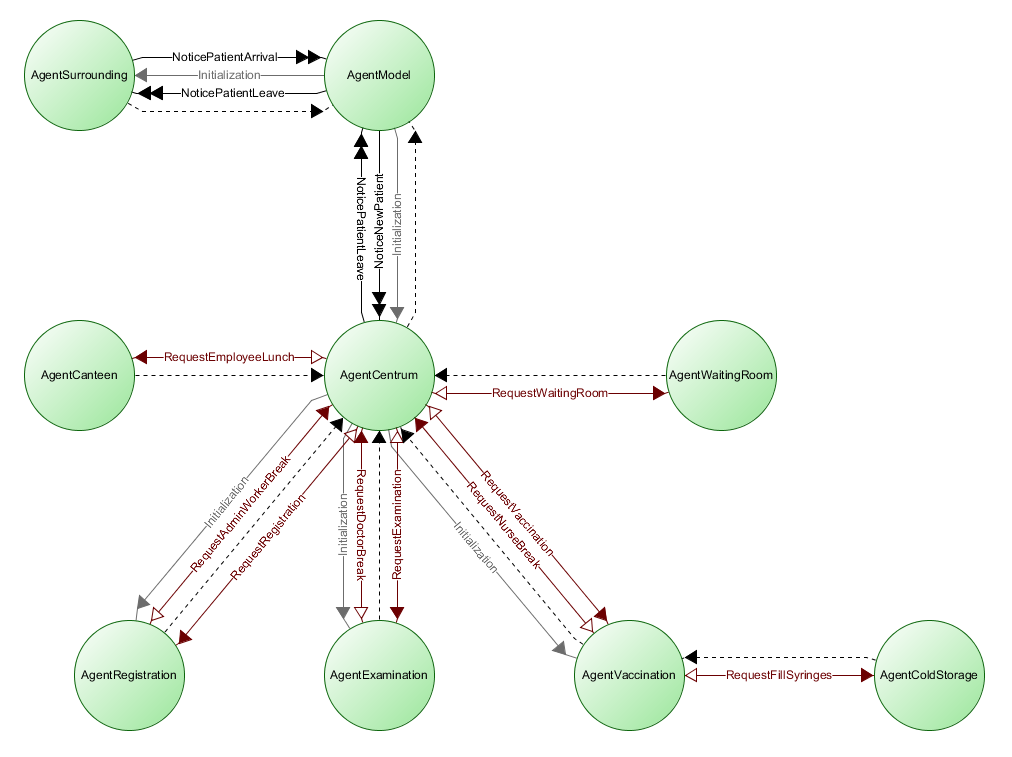
\includegraphics[width=\textwidth]{src/aba_architecture}
		\caption{Návrh agentovej architektúry vytvorený pomocou nástroja ABABuilder.}
	\end{figure}

	\subsubsection*{Hierarchická reprezentácia agentov}
	\begin{itemize}
		\item AgentModel (boss)
		\begin{itemize}
			\item[$	\triangleright $] AgentSurrounding
			\item[$	\triangleright $] AgentCentrum
			\begin{itemize}
				\item[$	\triangleright $] AgentRegistration
				\item[$	\triangleright $] AgentExamination
				\item[$	\triangleright $] AgentVaccination
				\begin{itemize}
					\item[$	\triangleright $] AgentColdStorage
				\end{itemize}
				\item[$	\triangleright $] AgentWaitingRoom
				\item[$	\triangleright $] AgentCanteen
			\end{itemize}
		\end{itemize}
	\end{itemize}
	
	\newpage
	
	\subsection{Agenti}
	
	\subsubsection{AgentModel}
	
	Agent modelu reprezentuje najvyššieho agenta (boss agent) v agentovej štruktúre. Zabezpečuje inicializáciu agenta okolia (\textbf{AgentSurrounding}) a agenta centra (\textbf{AgentCentrum}). Okrem toho iba preposiela správy medzi agentom okolia a agentom centra o príchode (odchode) pacienta.
	
	\vspace{0.8cm}
	
	\begin{figure}[hbt!]
		\centering
		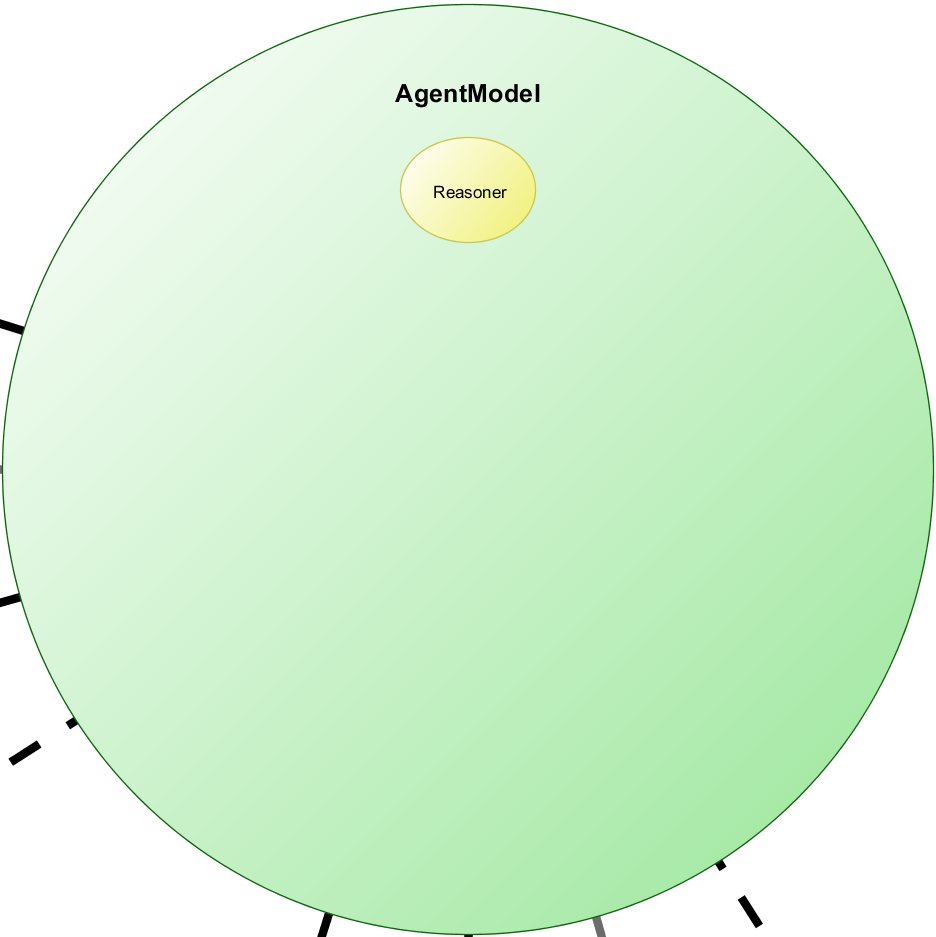
\includegraphics[width=0.6\textwidth]{src/AgentModel}
		\caption{Vnútorná štruktúra agenta modelu.}
	\end{figure}

	\newpage
	
	\subsubsection{AgentSurrounding}
	
	Agent okolia má na starosť generovanie prichádzajúcich pacientov pomocou plánovača \textbf{SchedulerPatietsArrival}. Akcia \textbf{ActionCancelPatients} vyberie z objednaných pacientov tých, ktorý sa vakcinácie nemôžu zúčastniť. Pre účely experimentu č. 3 existuje ešte akcia \textbf{ActionPatientsWithEarlyArrival}, ktorá vygeneruje všetkých objednaných pacientov už aj s so skorším časom príchodu ako je ich plánovaný. Takto vygenerovaní pacienti sa vložia do prioritného frontu s prioritou času ich príchodu do systému. Ten zabezpečuje takisto plánovač \textbf{SchedulerPatietsArrival}.
	
	Agent okolia taktiež ukončuje replikáciu za podmienky, že aktuálny simulačný čas je väčší než doba otvorenia centra a zároveň všetci objednaní a príchodzí pacienti boli zaočkovaní.
	
	Obsahuje náhodné generátory pre potreby rušenia pacientov a ich prípadných skorších príchodov.
	
	\vspace{0.8cm}
	
	\begin{figure}[hbt!]
		\centering
		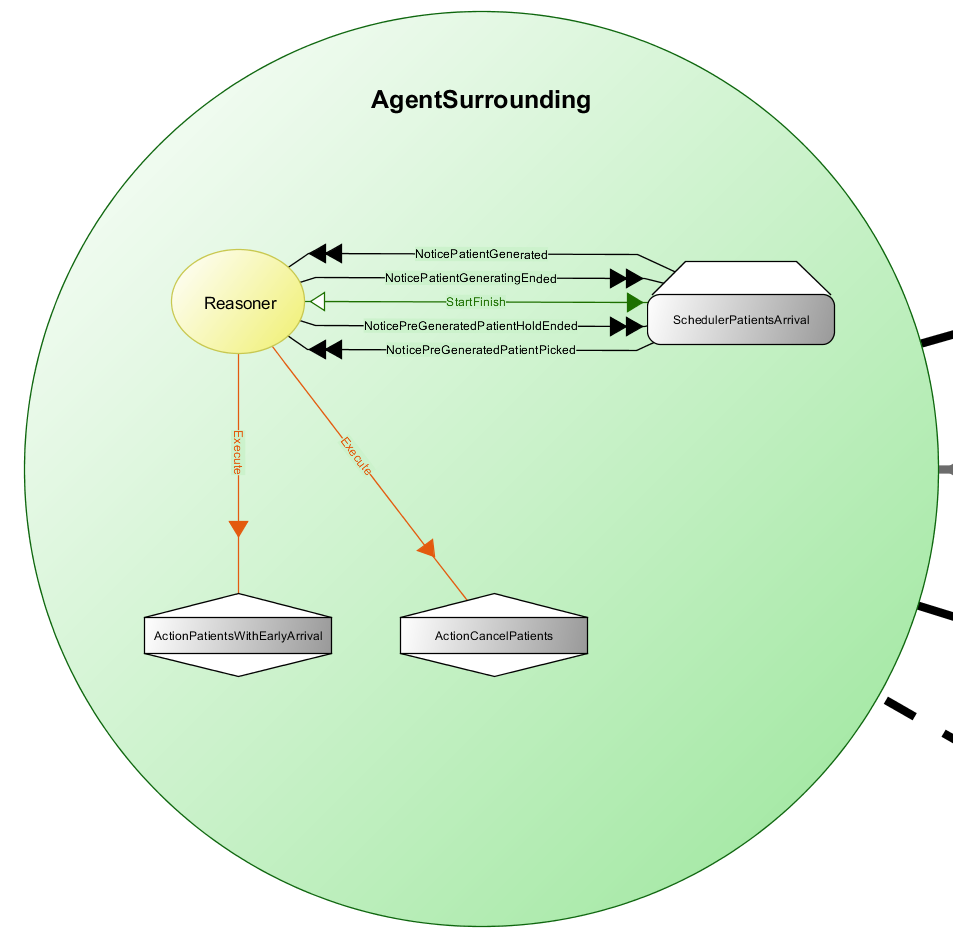
\includegraphics[width=0.7\textwidth]{src/AgentSurrounding}
		\caption{Vnútorná štruktúra agenta okolia.}
	\end{figure}
	
	\newpage
	
	\subsubsection{AgentCentrum}
	
	Agent centra zabezpečuje prechod pacienta (zamestnancov) systémom pomocou správ typu \textit{Request-Response} jednotlivým miestnostiam so zamestnancami vakcinačného centra. Je sprostredkovateľom presunu zamestnancov do jedálne na obednú prestávku. Okrem toho zabezpečuje aj ich presuny medzi miestnosťami, na čo využíva okamžitých asistentov \textbf{ProcessMovingRegToExa}, \textbf{ProcessMovingExaToVac} a \textbf{ProcessMovingVacToWai}. Akcia \textbf{ProcessMovingToFromCan} modeluje presun zamestnancov vakcinačného centra do a z jedálne.
	
	Udržuje aktuálne informácie o presúvajúcich sa entitách (pacienti aj zamestnanci) a obsahuje náhodné generátory pre potreby modelovania presunov centrom.
	
	\vspace{0.8cm}
	
	\begin{figure}[hbt!]
		\centering
		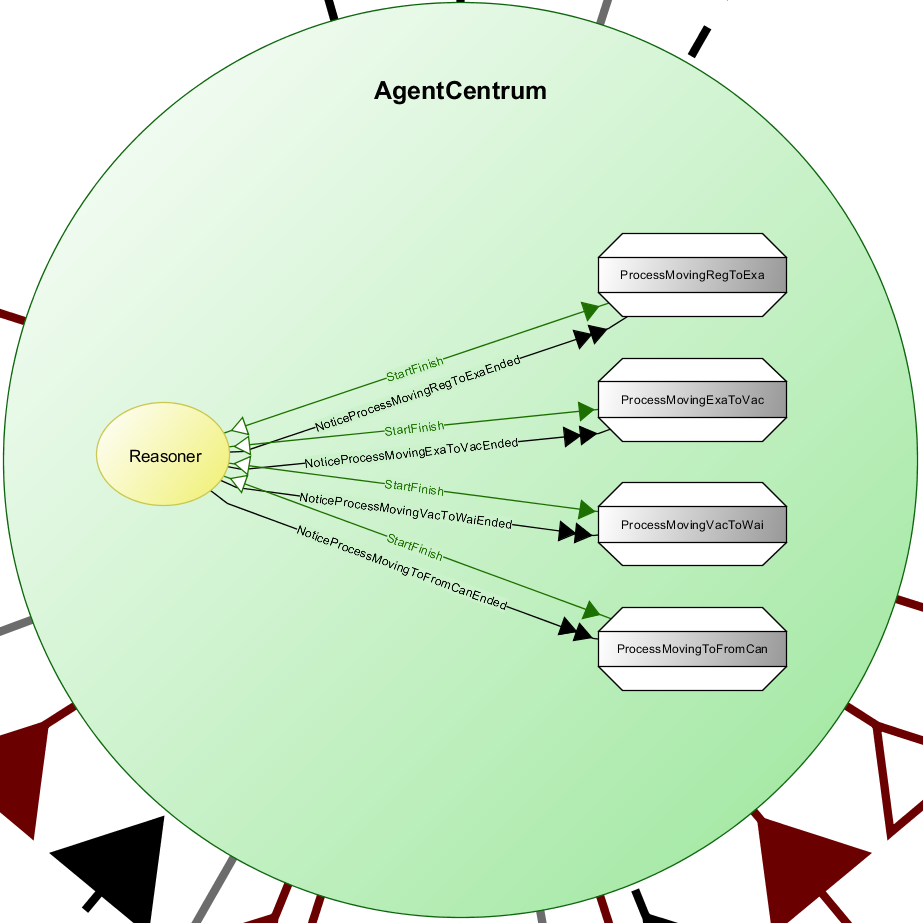
\includegraphics[width=0.7\textwidth]{src/AgentCentrum}
		\caption{Vnútorná štruktúra agenta centra.}
	\end{figure}
	
	\newpage
	
	\subsubsection{AgentRegistration}
	
	Agent registrácie predstavuje miestnosť registrácie s administratívnymi pracovníkmi. Je zodpovedný za vykonanie registrácie pacienta - proces \textbf{ProcessRegistration} a naplánovanie obednej prestávky pre pracovníkov - plánovač \textbf{SchedulerAdminWorkerBreak}. 
	
	Obsahuje taktiež rad, do ktorého sa zaraďujú pacienti, pre ktorých momentálne nie je voľný administratívny pracovník a udržuje si štatistiky o dĺžke radu pred registráciou a o dĺžke čakania v ňom.
	
	Poskytuje náhodný generátor pre náhodné zvolenie voľného pracovníka. Generátor pre dĺžku registrácie obsahuje už samotná entita pracovník.
	
	\vspace{0.8cm}
	
	\begin{figure}[hbt!]
		\centering
		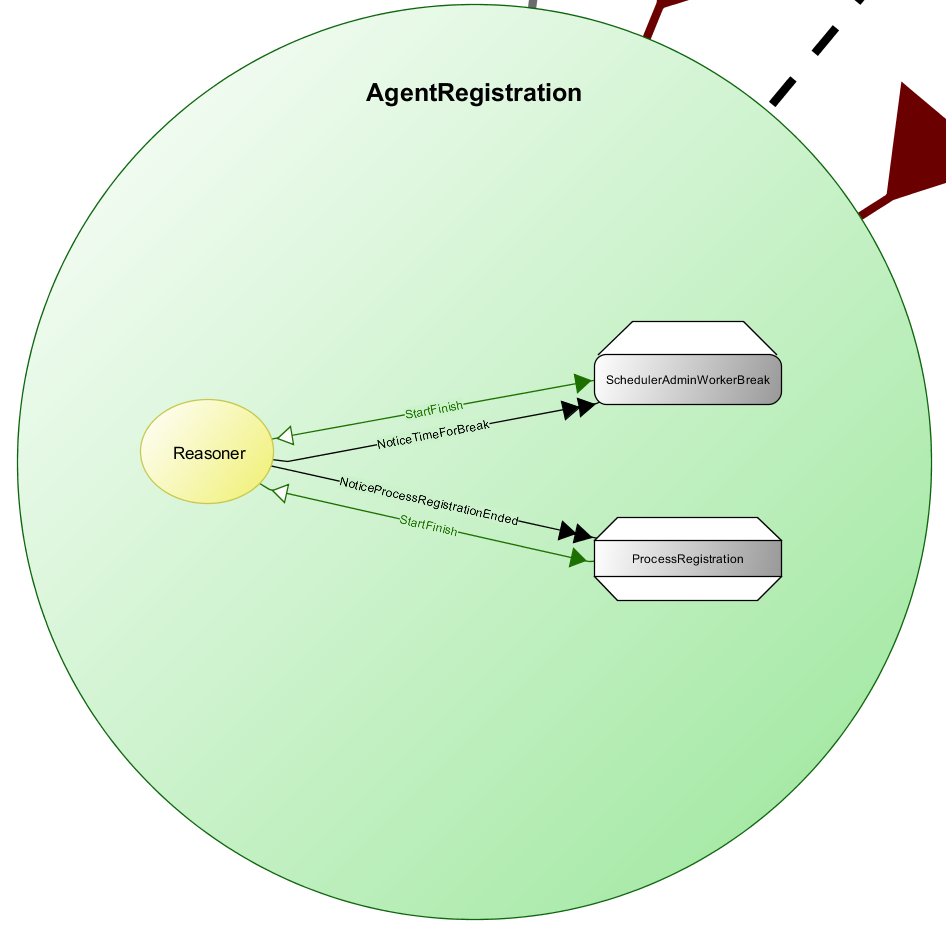
\includegraphics[width=0.7\textwidth]{src/AgentRegistration}
		\caption{Vnútorná štruktúra agenta registrácie.}
	\end{figure}
	
	\newpage
	
	\subsubsection{AgentExamination}
	
	Agent vyšetrenia reprezentuje miestnosť pre lekárske vyšetrenie doktorom. Je zodpovedný za vykonanie vyšetrenia pacienta a určenia dĺžky pobytu v čakárni - proces \textbf{ProcessExamination} a naplánovanie obednej prestávky pre doktorov - plánovač \textbf{SchedulerDoctorBreak}. 
	
	Obsahuje taktiež rad, do ktorého sa zaraďujú pacienti, pre ktorých momentálne nie je voľný doktor a udržuje si štatistiky o dĺžke radu pred vyšetrením a o dĺžke čakania v ňom.
	
	Poskytuje náhodný generátor pre náhodné zvolenie voľného doktora. Generátor pre dĺžku vyšetrenia a voľby o dĺžke zotrvania v čakárni obsahuje už samotná entita doktora.
	
	\vspace{0.8cm}
	
	\begin{figure}[hbt!]
		\centering
		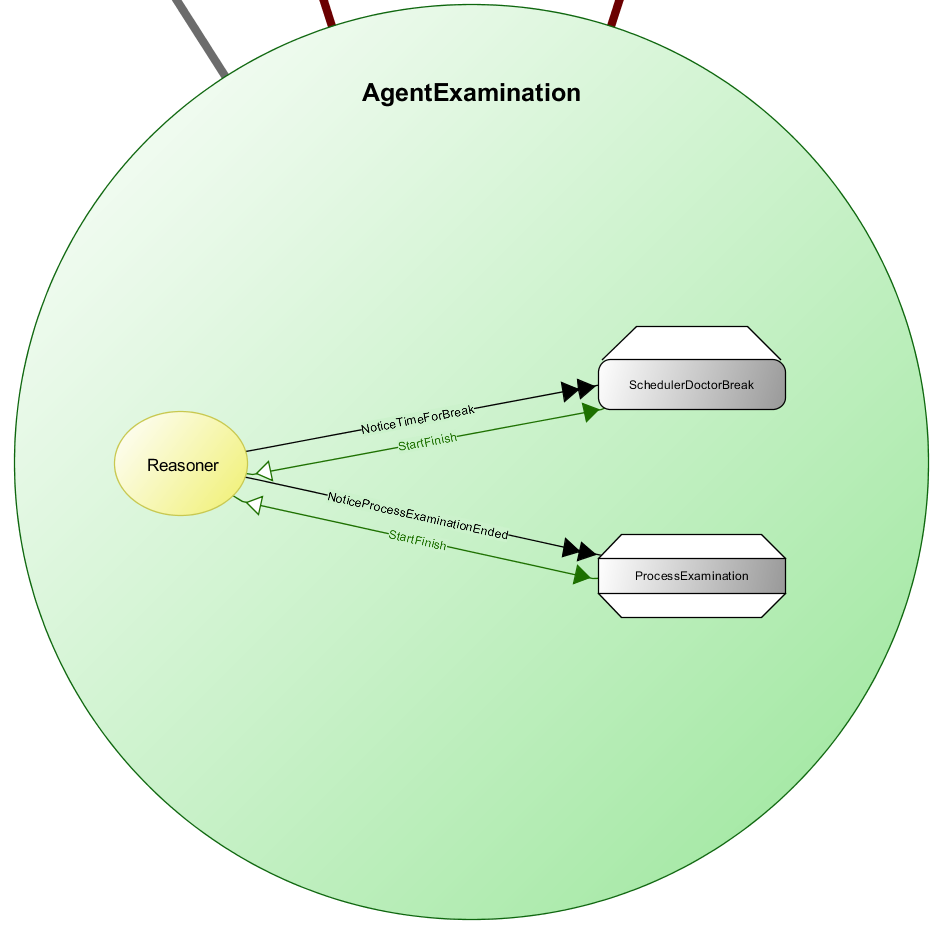
\includegraphics[width=0.7\textwidth]{src/AgentExamination}
		\caption{Vnútorná štruktúra agenta vyšetrenia.}
	\end{figure}
	
	\newpage
	
	\subsubsection{AgentVaccination}
	
	Agent vakcinácie modeluje miestnosť pre vakcináciu zdravotnými sestrami. Je zodpovedný za vykonanie vakcinácie  - proces \textbf{ProcessVaccination}, naplánovanie obednej prestávky pre zdravotné sestry - plánovač \textbf{SchedulerNurseBreak} a proces presunu zdravotnej sestry do miestnosti s chladiacim zariadením - \textbf{ProcessMovingToFromColdStor}.
	
	Obsahuje taktiež rad, do ktorého sa zaraďujú pacienti, pre ktorých momentálne nie je voľná zdravotná sestra a udržuje si štatistiky o dĺžke radu pred vyšetrením a o dĺžke čakania v ňom.
	
	Nachádza sa v ňom náhodný generátor pre náhodné zvolenie voľnej zdravotnej sestry a generátor pre modelovanie dĺžky presunu do miestnosti pre napĺňanie striekačiek. Generátor pre dĺžku očkovania obsahuje už samotná entita zdravotnej sestry.
	
	\vspace{0.8cm}
	
	\begin{figure}[hbt!]
		\centering
		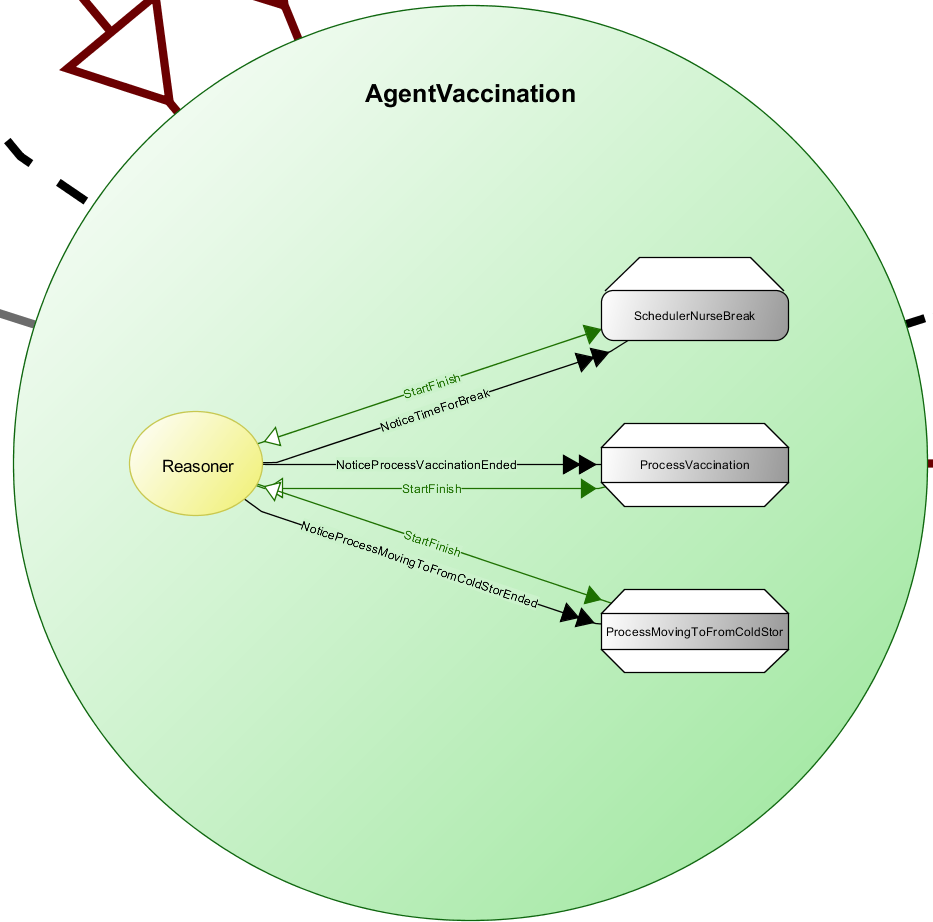
\includegraphics[width=0.7\textwidth]{src/AgentVaccination}
		\caption{Vnútorná štruktúra agenta vakcinácie.}
	\end{figure}
	
	\newpage
	
	\subsubsection{AgentColdStorage}
	
	Agent miestnosti s chladiacim zariadením predstavuje miestnosť kam si zdravotné sestry chodia dopĺňať striekačky s vakcínami. Agent zabezpečuje za vykonanie naplnenia striekačiek  - proces \textbf{ProcessFillingSyringes}.
	
	Obsahuje rad, do ktorého sa zaraďujú zdravotné sestry, pokiaľ sú už v miestnosti aspoň 2 sestry. Pre tento rad udržuje štatistiky o jeho dĺžke.
	
	Nachádza sa v ňom náhodný generátor pre náhodné zvolenie voľnej zdravotnej sestry a generátor pre modelovanie dĺžky presunu do miestnosti pre napĺňanie striekačiek. Generátor pre dĺžku napĺňania jednej striekačky obsahuje už samotná entita zdravotnej sestry.
	
	\vspace{0.8cm}
	
	\begin{figure}[hbt!]
		\centering
		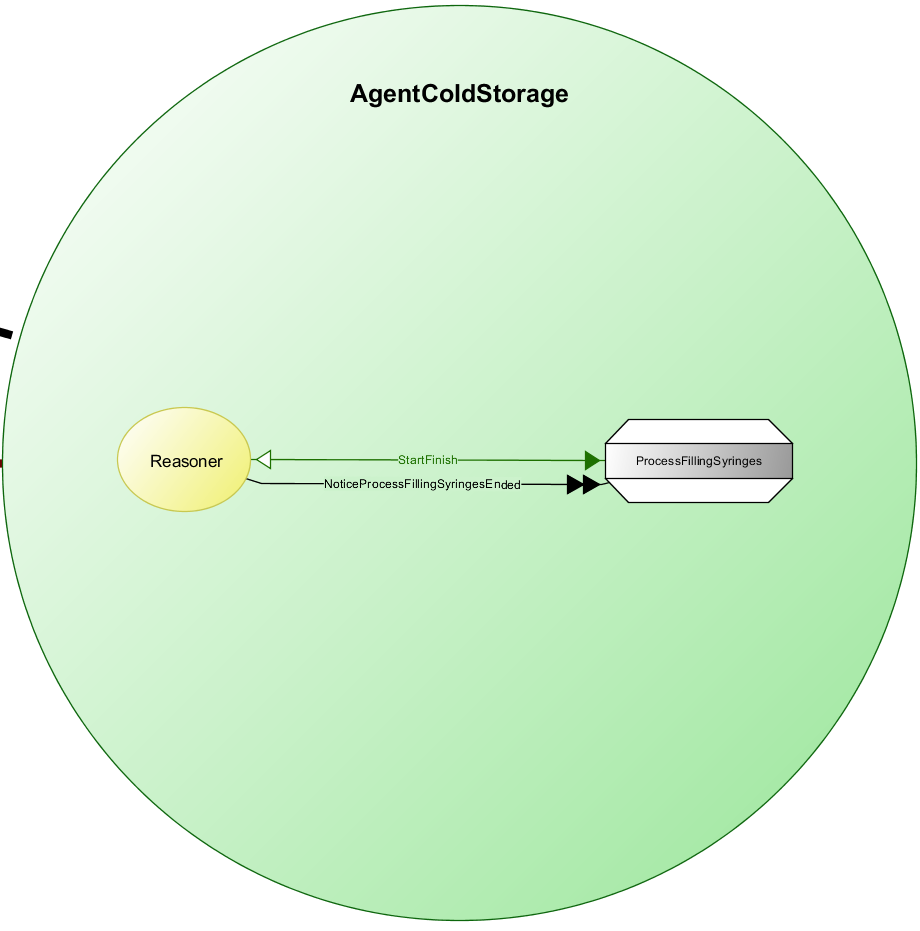
\includegraphics[width=0.7\textwidth]{src/AgentColdStorage}
		\caption{Vnútorná štruktúra agenta miestnosti s chladiacim zariadením.}
	\end{figure}
	
	\newpage
	
	\subsubsection{AgentWaitingRoom}
	
	Agent čakárne modeluje miestnosť čakárne. Je zodpovedný za vykonanie procesu čakania v čakárni čas stanovený doktorom pri lekárskom vyšetrení - \textbf{ProcessWaitingRoom}.
	
	Obsahuje informácie o aktuálnom stave čakárne a udržiava si štatistiky o počte pacientov v nej.
	
	\vspace{0.8cm}
	
	\begin{figure}[hbt!]
		\centering
		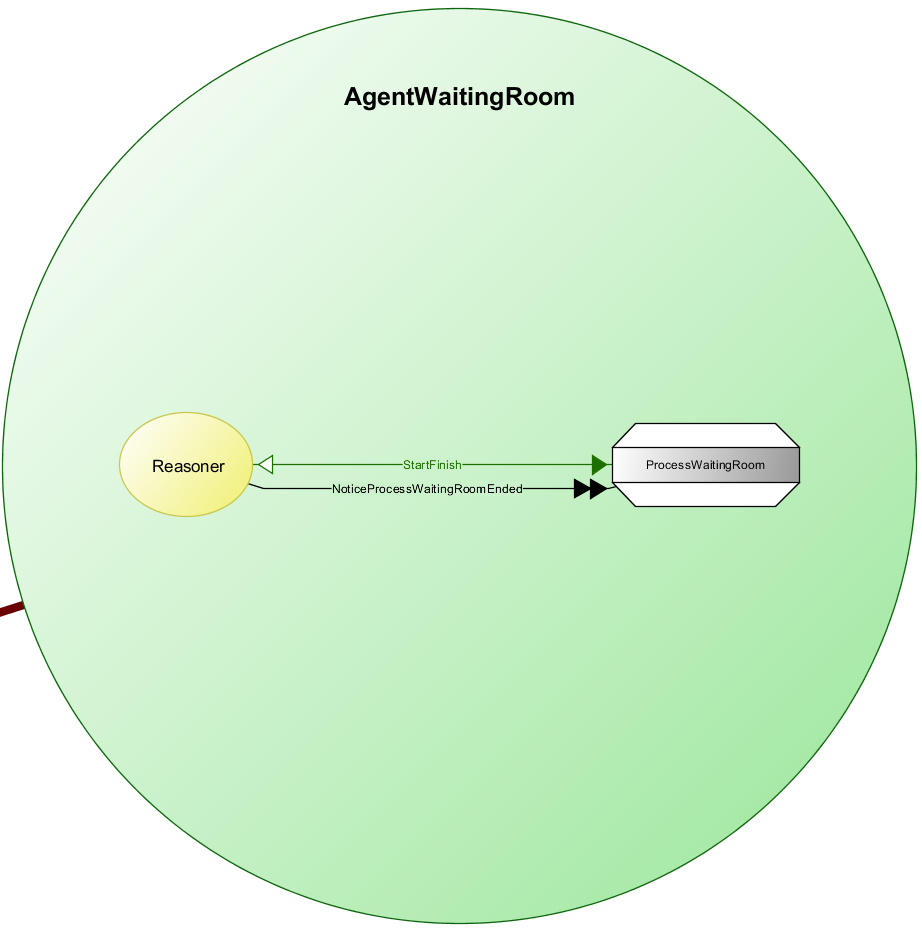
\includegraphics[width=0.7\textwidth]{src/AgentWaitingRoom}
		\caption{Vnútorná štruktúra agenta čakárne.}
	\end{figure}
	
	\newpage
	
	\subsubsection{AgentCanteen}
	
	Agent jedálne predstavuje miestnosť jedálne, kam sa pracovníci počas obednej prestávky chodia najesť. Je zodpovedný za modelovanie procesu jedenia - \textbf{ProcessEating}.
	
	Obsahuje informácie o aktuálnom stave jedálne.
	
	Poskytuje náhodný generátor pre modelovanie dĺžky procesu jedenia.
	
	\vspace{0.8cm}
	
	\begin{figure}[hbt!]
		\centering
		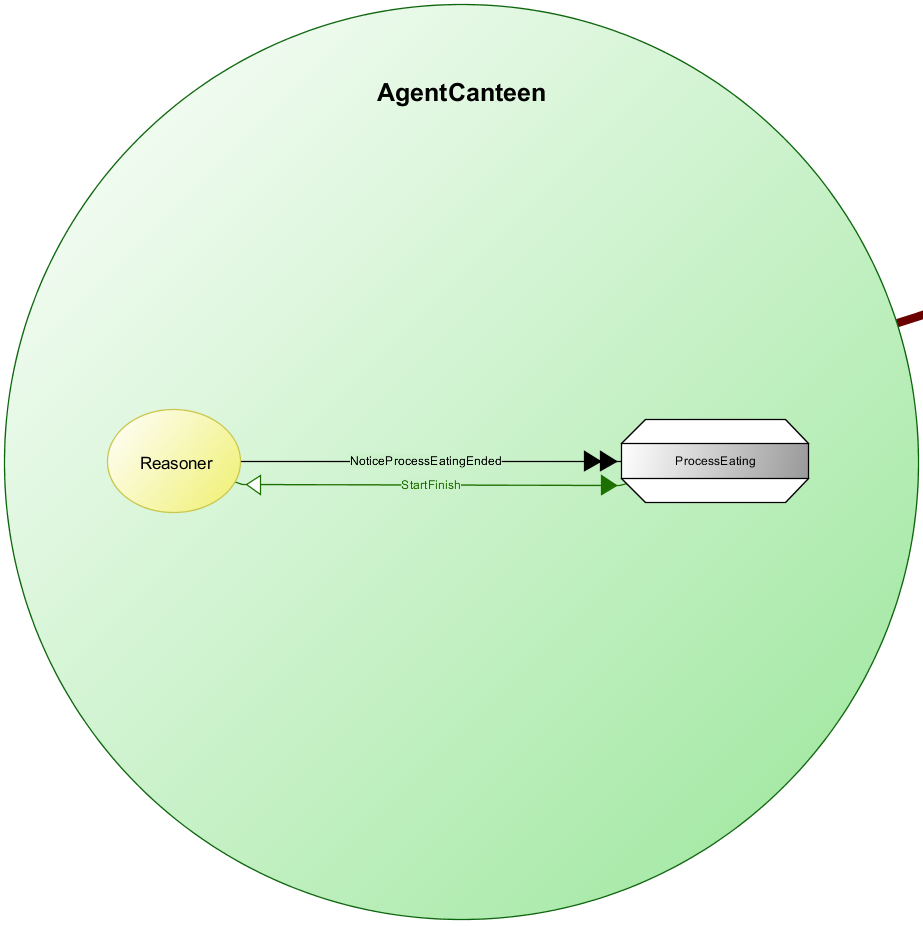
\includegraphics[width=0.7\textwidth]{src/AgentCanteen}
		\caption{Vnútorná štruktúra agenta jedálne.}
	\end{figure}
	
	\newpage
	
	\subsection{Entity}
	
	\subsubsection{EntityPatient}
	
	Entita predstavujúca pacienta. Obsahuje premenné definujúce vlastnosti potrebné pre štatistické vyhodnotenia, či generovanie - čas príchodu, časy začiatku čakania v radoch na registráciu, vyšetrenie a očkovanie a čas pobytu v čakárni.
	
	\subsubsection{VaccineCentrumEntity}
	
	Všeobecná entita zamestnanca vakcinačného centra. Obsahuje premenné definujúce jej aktuálny stav, priemerné vyťaženie, informáciu o tom, či zamestnanec už mal obednú prestávku a niekoľko ďalších. Poskytuje metódy pre priradenie pacienta zamestnancovi, či jeho uvoľnení. Jeho potomkami sú prirodzene:
	\begin{itemize}
		\item Administratívny pracovník (\textbf{EntityAdminWorker})
		\begin{itemize}
			\item obsahuje náhodný generátor pre modelovanie trvania procesu registrácie
		\end{itemize}
		\item Doktor (\textbf{EntityDoctor})
		\begin{itemize}
			\item obsahuje náhodný generátor pre modelovanie trvania procesu vyšetrenia a generátor pre voľbu doktora o dĺžke pobytu pacienta v čakárni
		\end{itemize}
		\item Zdravotná sestra (\textbf{EntityNurse})
		\begin{itemize}
			\item obsahuje náhodný generátor pre modelovanie trvania procesu vakcinácie a procesu napĺňania injekčnej striekačky a informáciu o počte striekačiek k dispozícii
		\end{itemize}
	\end{itemize}

	\subsubsection{Pool}
	
	Pomocná štruktúra pre prácu s entitami zamestnancov centra. Poskytuje údaje o počte voľných (zaneprázdnených pracovníkoch) a o ich priemernej vyťaženosti. Ponúka možnosť priradenia voľného pracovníka pacientov, či jeho uvoľnenie.
	
	Štruktúra je použitá v agentoch \textbf{AgentRegistration}, \textbf{AgentExamination} a \textbf{AgentVaccination}.
	
	\subsection{Správy}
	
	V modeli sú použité správy 3 druhov \textbf{MessagePatient}, pre správy týkajúce sa pacientov, \textbf{MessageNurse} pre správy o presune a napĺňaní striekačiek zdravotnými sestrami a \textbf{MessageBreak} pre správy týkajúce sa obednej prestávky zamestnancov.
	
	\section{Validácia}
	
	Pre validáciu agentového modelu bude použitý už skôr vytvorený udalostný model. Ten modeluje vakcinačné centrum bez modelovania presunov pacientov, bez obedných prestávok zamestnancov a bez procesu napĺňania injekčných striekačiek zdravotnými sestrami. V agentovom modeli boli trvania všetkých vyššie spomenutých procesov nastavené na 0, aby boli zabezpečené rovnaké podmienky.
	
	\subsubsection*{Parametre modelu} 
	\begin{itemize}
		\item 540 objednaných pacientov
		\item 5 administratívnych pracovníkov
		\item 6 doktorov
		\item 3 zdravotné sestry
	\end{itemize}
	
	\subsubsection*{Udalostne-orientovaný model}
	
	\noindent\begin{tabular}{ll}
		\textbf{Počet replikácií} & 1 000 000 \\
	\end{tabular}
	
	\begin{table}[hbt!]
		\begin{tabular}{l|lll}
			& \textbf{Dĺžka radu} & \textbf{Čas čakania v rade} & \textbf{Vyťaženosť entít} \\
			\hline
			\textbf{Registrácia} 	& 0                   & 0                           & 0,547300                  \\
			\textbf{Vyšetrenie}  	& 0,155953            & 13,353532                   & 0,658576                  \\
			\textbf{Vakcinácia}  	& 0,006110            & 1,315286                    & 0,329381                 
		\end{tabular}
	\end{table}
	
	Priemerný počet čakajúcich pacientov v čakárni bol \textbf{14,365139} s 95\% intervalom spoľahlivosti (14,364539; 14,365739).
	
	\subsubsection*{Agentovo-orientovaný model}
	
	\noindent\begin{tabular}{ll}
		\textbf{Počet replikácií} & 10 000 \\
	\end{tabular}
	
	\begin{table}[hbt!]
		\begin{tabular}{l|lll}
			& \textbf{Dĺžka radu} & \textbf{Čas čakania v rade} & \textbf{Vyťaženosť entít} \\
			\hline
			\textbf{Registrácia} 	& 0                   & 0                           & 0,552961                  \\
			\textbf{Vyšetrenie}  	& 0,203721            & 13,281058                   & 0,665432                  \\
			\textbf{Vakcinácia}  	& 0,020161            & 1,314890                    & 0,334489                 
		\end{tabular}
	\end{table}
	
	Priemerný počet čakajúcich pacientov v čakárni bol \textbf{14,485763} s 95\% intervalom spoľahlivosti (14,480371; 14,491155).
	
	Porovnanie ukazuje, že výsledky sa líšia len minimálne. To môže byť dôsledkom použitia iných generátorov náhodných čísel, ale aj iného prístupu k modelovaniu systému. Na základe porovnania, môžme považovať model za \textbf{validný}.
	
	\section{Experimenty}
	
	\subsection{Experiment: Súčasný stav}
	
	V súčasnosti pracuje vo vakcinačnom centre \textbf{5 administratívnych pracovníkov}, \textbf{6 lekárov} a \textbf{3 zdravotné sestry}. Na deň je objednaných \textbf{540 pacientov} - na každú minútu 1. Pacienti prichádzajú presne v čase, na kedy sú objednaní. Namodelujte súčasné fungovanie centra. 
	
	\subsection*{Vyhodnotenie (10 000 replikácií)}

	\subsubsection*{Dĺžka radu}

	\begin{table}[hbt!]
		\begin{tabular}{p{6cm}|p{4.5cm}p{4.5cm}}
			& \textbf{Výsledná hodnota} & \textbf{95\% interval spoľahlivosti} \\
			\hline\hline
			\textbf{Registrácia} 	& 0,025536            & (0,025267; 0,025805)			
			\\\hline
			\textbf{Vyšetrenie}  	& 1,039960            & (1,027388; 1,051991)	
			\\\hline
			\textbf{Vakcinácia}  	& 0,173967            & (0,172625; 0,175308)
		\end{tabular}
	\end{table}

	\subsubsection*{Čas čakania v rade (s)}
	
	\begin{table}[hbt!]
		\begin{tabular}{p{6cm}|p{4.5cm}p{4.5cm}}
			& \textbf{Výsledná hodnota} & \textbf{95\% interval spoľahlivosti} \\
			\hline\hline
			\textbf{Registrácia} 	& 1,673095            & (1,655552; 1,690637)			
			\\\hline
			\textbf{Vyšetrenie}  	& 68,141699           & (67,337374; 68,946024)	
			\\\hline
			\textbf{Vakcinácia}  	& 11,405330           & (11,317642; 11,493019)
		\end{tabular}
	\end{table}

	\subsubsection*{Vyťaženosť zamestnancov centra}
	
	\begin{table}[hbt!]
		\begin{tabular}{p{6cm}|p{4.5cm}p{4.5cm}}
			& \textbf{Výsledná hodnota} & \textbf{95\% interval spoľahlivosti} \\
			\hline\hline
			\textbf{Administratívny pracovníci} 	& 0,576696            & (0,576459; 0,576933)			
			\\\hline
			\textbf{Doktori}  						& 0,663062            & (0,662491; 0,663634)	
			\\\hline
			\textbf{Zdravotné sestry}  				& 0,454007            & (0,453745; 0,454268)
		\end{tabular}
	\end{table}

	\newpage

	\subsubsection*{Ďalšie štatistiky}
	
	\begin{table}[hbt!]
		\begin{tabular}{p{6cm}|p{4.5cm}p{4.5cm}}
			& \textbf{Výsledná hodnota} & \textbf{95\% interval spoľahlivosti} \\
			\hline\hline
			\textbf{Počet pacientov v čakárni} 								& 14,408798           & (14,403821; 14,413776)			
			\\\hline
			\textbf{Dĺžka radu pred miestnosťou s chladiacim zariadením}	& 0,002751            & (0,002678; 0,002823)	
			\\\hline
			\textbf{Nadčas (hh:mm:ss)}										& 00:33:50,883        & (00:33:43,557; 00:33:58,209)
			\\\hline
			\textbf{Priemerná vyťaženosť všetkých zamestnancov}  			& 0,564588            & (0,564336; 0,564841)
			\\\hline
			\textbf{Priemerný čas čakania vo všetkých radoch (hh:mm:ss)}	& 00:01:21,220        & (00:01:20,379; 00:01:22,061)
		\end{tabular}
	\end{table}

	\subsection{Experiment: Súčasný stav so skoršími príchodmi pacientov}
	
	V súčasnosti pracuje vo vakcinačnom centre \textbf{5 administratívnych pracovníkov}, \textbf{6 lekárov} a \textbf{3 zdravotné sestry}. Na deň je objednaných \textbf{540 pacientov}. Niektorí ľudia prichádzajú na očkovanie z väčšej vzdialenosti a najmä z tohto dôvodu príde časť osôb skôr ako je objednaná. Bolo zistené, že iba \textbf{10\% osôb} sa dostaví na očkovanie \textbf{v presne stanovenom} čase. Ostatní sa dostavia vopred pričom čas o koľko skôr prídu môžeme modelovať pomocou spojitého empirického rozdelenia pravdepodobnosti: 
	\begin{itemize}
		\item $ \left\langle 1, 20 \right) $ min; $ p = 0.3 $
		\item $ \left\langle 20, 60 \right) $ min; $ p = 0.4 $
		\item $ \left\langle 60, 80 \right) $ min; $ p = 0.2 $
		\item $ \left\langle 80, 240 \right) $ min; $ p = 0.1 $
	\end{itemize}
	
	\subsection*{Vyhodnotenie (10 000 replikácií)}
	
	\subsubsection*{Dĺžka radu}
	
	\begin{table}[hbt!]
		\begin{tabular}{p{6cm}|p{4.5cm}p{4.5cm}}
			& \textbf{Výsledná hodnota} & \textbf{95\% interval spoľahlivosti} \\
			\hline\hline
			\textbf{Registrácia} 	& 2,487781            & (2,478820; 2,496743)			
			\\\hline
			\textbf{Vyšetrenie}  	& 3,105683            & (3,077597; 3,133770)	
			\\\hline
			\textbf{Vakcinácia}  	& 0,338557            & (0,336113; 0,341002)
		\end{tabular}
	\end{table}

	\newpage
	
	\subsubsection*{Čas čakania v rade (s)}
	
	\begin{table}[hbt!]
		\begin{tabular}{p{6cm}|p{4.5cm}p{4.5cm}}
			& \textbf{Výsledná hodnota} & \textbf{95\% interval spoľahlivosti} \\
			\hline\hline
			\textbf{Registrácia} 	& 160,089793          & (159,520636; 160,658949)			
			\\\hline
			\textbf{Vyšetrenie}  	& 199,778530          & (197,979708; 201,577352)	
			\\\hline
			\textbf{Vakcinácia}  	& 21,783831           & (21,627307; 21,940356)
		\end{tabular}
	\end{table}
	
	\subsubsection*{Vyťaženosť zamestnancov centra}
	
	\begin{table}[hbt!]
		\begin{tabular}{p{6cm}|p{4.5cm}p{4.5cm}}
			& \textbf{Výsledná hodnota} & \textbf{95\% interval spoľahlivosti} \\
			\hline\hline
			\textbf{Administratívny pracovníci} 	& 0,573646            & (0,573374; 0,573919)			
			\\\hline
			\textbf{Doktori}  						& 0,675411            & (0,674805; 0,676017)	
			\\\hline
			\textbf{Zdravotné sestry}  				& 0,462365            & (0,462085; 0,462645)
		\end{tabular}
	\end{table}
	
	\subsubsection*{Ďalšie štatistiky}
	
	\begin{table}[hbt!]
		\begin{tabular}{p{6cm}|p{4.5cm}p{4.5cm}}
			& \textbf{Výsledná hodnota} & \textbf{95\% interval spoľahlivosti} \\
			\hline\hline
			\textbf{Počet pacientov v čakárni} 								& 14,680409           & (14,674967; 14,685851)			
			\\\hline
			\textbf{Dĺžka radu pred miestnosťou s chladiacim zariadením}	& 0,004639            & (0,004552; 0,004727)	
			\\\hline
			\textbf{Nadčas (hh:mm:ss)}										& 00:23:18,933        & (00:23:10,419; 00:23:27,447)
			\\\hline
			\textbf{Priemerná vyťaženosť všetkých zamestnancov}  			& 0,570474            & (0,570198; 0,570750)
			\\\hline
			\textbf{Priemerný čas čakania vo všetkých radoch (hh:mm:ss)}	& 00:06:21,652        & (00:06:19,679; 00:06:23,625)
		\end{tabular}
	\end{table}

	\subsection{Experiment: 1700 pacientov za deň}
	
	Upravte model tak, aby vakcinačné centrum obsluhovalo denne \textbf{1700 ľudí}. Stanovte také počty jednotlivých typov personálu, aby priemerné \textbf{vyťaženie} personálu neprekračovalo \textbf{70\%} a \textbf{sumárna priemerná doba čakania} osoby na jednotlivé úkony nepresiahla \textbf{15 minút}.
	
	Oproti pôvodným 540 pacientom znamená 1700 pacientov za deň približne \textbf{3,15 násobný nárast}. Navýšením počtov zamestnancov 3,15 násobne (16 administratívnych pracovníkov, 19 doktorov, 9 zdravotných sestier) dostaneme vyťaženie blízke pôvodnému stavu. Toto slúži ako bod, od ktorého môžme pokračovať v znižovaní stavov pracovníkov pre dosiahnutie žiadaných výsledkov.
	
	Pre zvýšenie celkovej priemernej vyťaženosti zamestnancov z pôvodných 56,5\% na požadovaných 70\% je potrebné znížiť kapacity personálu na úroveň približne 80\%. Pre personál to znamená zníženie stavov na 13 administratívnych pracovníkov, 15 doktorov a 7 zdravotných sestier, čo znamená aj proporcionálne zvýšenie ich vlastne vyťaženosti. Pre počet doktorov vykonáme experiment, ktorý ukáže závislosť celkového vyťaženia všetkých pracovníkov, počte ľudí v rade pred vyšetrením a celkovom čase strávenom čakaním vo všetkých radoch od počtu doktorov v centre.
	
	\section{Použité knižnice}
	
	\subsection*{OSPABA}
	
	\noindent Balíček knižníc pre prácu s agentovo orientovaým modelovaním.
	
	\subsection*{LiveCharts}
	
	\noindent Knižnica pre vykresľovanie grafov. \\
	Dostupná na https://lvcharts.net.
	
	\subsection*{OptimizedPriorityQueue}
	
	\noindent Knižnica pre implementáciu prioritného frontu. \\ 
	Dostupná na https://www.nuget.org/packages/OptimizedPriorityQueue/
	
\end{document}